\chapter{Methodology}
\label{sec:methodology}

This chapter outlines the seven-stage research method designed to create and assess a multimodal Automatic Personality Recognition (APR) framework for Filipino Instagram users. This framework will tackle the specific language and cultural challenges found in the dataset, including code switching and unique patterns of visual self-expression. The process starts with exploratory data analysis, followed by preprocessing and feature extraction from text, images, and metadata. It also includes an early combination of these features. Finally, we will train machine learning models and thoroughly evaluate them to see how well they perform in predicting outcomes.

\begin{figure}[H]
	\centering
	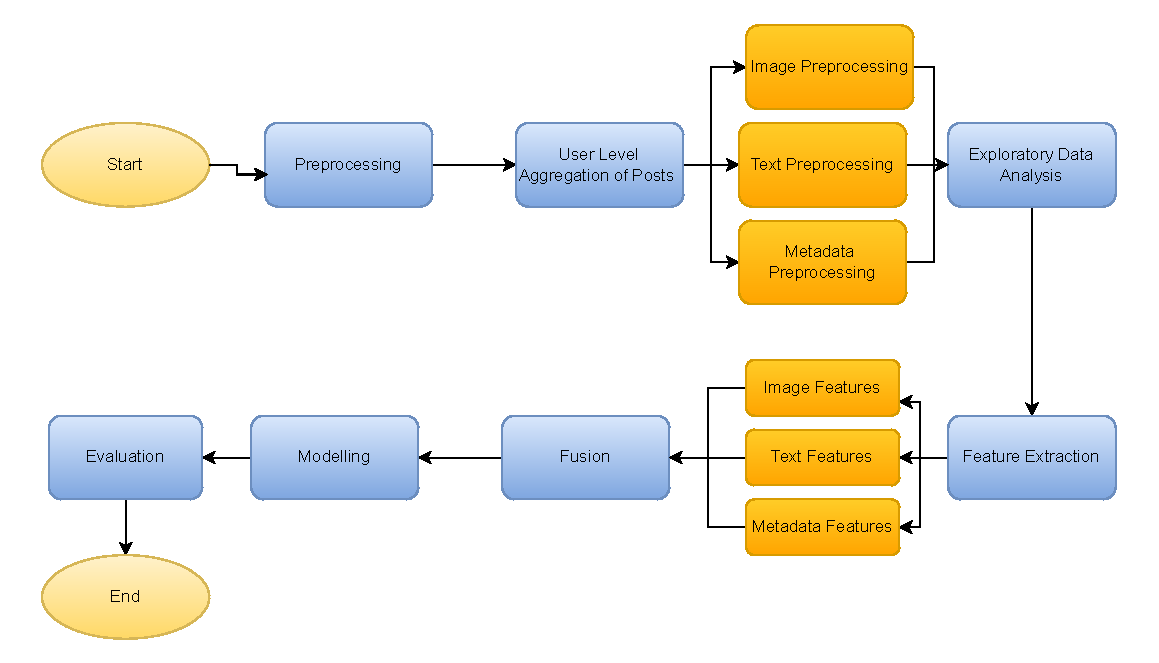
\includegraphics[width=\textwidth]{"figures/Methodology-Flowchart.pdf"}
	\caption{Methodology Flowchart}
	\label{fig:methodology_pipeline}
\end{figure}

\section{Data Source}
\label{sec:data}
This research is grounded in the Instagram subset of the PagkataoKo dataset, a comprehensive resource specifically curated for Filipino APR studies \citep{tighe_acorda_2022}. The dataset's inclusion of user-generated content (posts and images), demographic information, and self-reported Big Five personality scores makes it an ideal foundation for this supervised machine learning investigation. The original Instagram subset contains data from 1,380 participants who provided access to their accounts, totaling 195,757 posts.

\subsection{Data Collection Methodology}
The data was gathered between the first week of June 2019 and the second week of February 2020 through a purpose-built web application \citep{tighe_acorda_2022}. This tool streamlined the collection process by first presenting participants with a consent form and study directions. Upon granting consent, participants authorized the application to access their social media data via the official Instagram Legacy API. The application then collected post data (captions and image links) and account metadata. Following this automated collection, participants completed a demographic questionnaire and the 44-item Big Five Inventory (BFI-44) to assess their personality traits \citep{tighe_acorda_2022}.

\subsection{Participant Sampling and Filtering}
A mixed sampling strategy was employed to recruit participants. The initial phase utilized convenience and snowball sampling, where information about the study was disseminated within the researchers' immediate networks. To reach a broader Filipino audience, this was followed by a series of targeted online advertisement campaigns on Facebook, Instagram, and Twitter \citep{tighe_acorda_2022}.

From an initial pool of 3,186 participants, a filtering process was applied to ensure relevance to the Filipino context. Only individuals who identified their nationality as either "Filipino" or "mixed-Filipino" were retained, resulting in a final cohort of 3,128 individuals whose data comprises the full PagkataoKo dataset \citep{tighe_acorda_2022}.

\subsection{Ethical Clearance}
The entire data collection protocol, including the consent process and data handling procedures, was reviewed and granted ethical clearance by the Research Ethics Office of De La Salle University, Philippines. Participation was voluntary, with individuals providing informed electronic consent. The collection of social media data was conducted in strict accordance with the developer policies of Instagram at the time of collection \citep{tighe_acorda_2022}.

\subsection{Personality Score Transformation to Labels}
In its raw form, the PagkataoKo dataset provides personality scores as continuous numerical values ranging from 1.0 to 5.0 for each of the Big Five traits. Since this study frames personality recognition as a classification task, these continuous scores must be transformed into discrete labels.

To achieve this, a \textbf{median split} will be performed for each of the five personality traits independently. For a given trait (e.g., Openness), users with a score above the median value for that trait will be assigned the 'High' label (e.g., 'High-Openness'). Users with scores at or below the median will be assigned the 'Low' label (e.g., 'Low-Openness'). This process will result in five separate binary labeling schemes, one for each personality dimension, which will serve as the target variables for the classification models.

\subsection{Data Splitting}
For model training and evaluation, the dataset will be divided using a user-level stratified split for model training and evaluation: \textbf{70\%} for training, \textbf{15\%}for validation, and \textbf{15\%} for testing. To ensure that the proportion of 'High' and 'Low' labels for each personality trait is consistent across these sets, the split will be stratified based on the generated personality labels. This helps prevent model bias and ensures that the models are trained and evaluated on representative distributions of each personality class.

\section{Preprocessing}
This stage cleans and organizes the raw data to make it suitable for feature extraction. It is important to normalize multilingual text, manage platform-specific noise, and combine data into a usable format. The main task is \textbf{user-level aggregation}. Here, all posts, images, and metadata for a single user are collected into a single behavioral profile. This method lets the models learn from a user's digital footprint.

\subsection{Image Preprocessing}
All images will go through preprocessing to get them ready for the \textbf{ResNet50} model. Each image will be resized to 224x224 pixels to fit the model’s required input size. We will also check for corrupted image files. Any posts with unreadable images will be flagged and excluded from the image-based feature extraction process.

\subsection{Text Preprocessing}
A basic text cleaning method will be used to keep as much of the original content as possible, including multilingual text. The process will involve breaking down the raw caption text into tokens and replacing things like URLs and user mentions with generic tokens (e.g., URL, USER) instead of removing them completely. This way, we keep the context of where a link or mention appeared. All languages will be kept in the text.


\section{Exploratory Data Analysis}
\label{subsec:eda}

Before feature extraction, we will conduct exploratory data analysis (EDA) to understand the key features of the dataset. This analysis will aim to pinpoint demographic trends and content patterns that can guide feature engineering and model interpretation.

The demographic distribution of the final 1,300-user subset, as derived from the PagkataoKo dataset paper, is summarized in Table 4.1. The data shows a user base that is predominantly young (49.3\% aged 18-20) and female (78.0\%). Linguistically, captions are overwhelmingly English-dominant (75.6\%), with a smaller portion being Tagalog-dominant (4.3\%) or exhibiting code-switching (19.4\%).

\begin{table}[h]
	\centering
	\caption{Demographic distribution of Instagram subset (n=1,300)}
	\label{tab:demo}
	\begin{tabular}{lcc}
		\hline
		\textbf{Characteristic} & \textbf{Category} & \textbf{Percentage} \\ \hline
		\textbf{Age} & 18-20 & 49.3\% \\
		& 21-23 & 31.3\% \\
		& 24-26 & 10.7\% \\
		& $\geq$27 & 8.8\% \\ \hline
		\textbf{Sex} & Female & 78.0\% \\
		& Male & 20.0\% \\
		& Intersex/ Declined & 2.0\% \\ \hline
		\textbf{Language} & English-dominant & 75.6\% \\
		& Tagalog-dominant & 4.3\% \\
		& Code-switched & 19.4\% \\ \hline
	\end{tabular}
\end{table}

% --- REVISION G START: Added new section for PCA Rationale ---


\section{Feature Engineering}
\label{subsec:features}
This stage converts the raw, multimodal data associated with each Instagram user—comprising images, textual captions, and account metadata—into a single, quantitative feature vector. This vector is designed to be processed by supervised machine learning algorithms (logistic regression, support vector machines, and XGBoost) for the task of personality trait prediction. The process is divided into three parallel pipelines, one for each data modality, to ensure a clear and reproducible workflow.

\subsection{Image Modality Pipeline}
This pipeline processes all valid images from a user's profile to extract a comprehensive set of visual features. For each image, the following features are extracted in parallel before being aggregated to the user level.

\subsubsection{High-Level Semantic Features via ResNet50}
The pre-trained \textbf{ResNet50} convolutional neural network is used as a feature extractor. For each image, a \textbf{2,048-dimension feature vector} is extracted from the output of the final average pooling layer. This vector captures abstract visual concepts, objects, and textures.

ResNet50 was chosen because it demonstrates higher classification accuracy on benchmark datasets like ImageNet, is substantially more efficient in terms of model size (98 MB vs. 549 MB for VGG19), and its residual connections allow for the effective training of deeper networks, enabling the model to learn more complex feature representations without suffering from the vanishing gradient problem that can affect older architectures \citep{he2015, simonyan2014very}.

\subsubsection{Object and Scene Recognition via the Imagga API}
To quantify the semantic content and social context of the images, this study leverages the \textbf{Imagga API}, a commercial computer vision service.

Imagga is a cloud-based service that provides a suite of powerful image analysis tools through a simple API. Its core functions include automated image tagging, categorization, color extraction, and content moderation, all powered by pre-trained deep learning models capable of recognizing thousands of objects, scenes, and concepts \citep{imagga_website, imagga_solutions}. The Imagga API was selected for its robust, recognition capabilities, which provide a reliable method for extracting semantic features without the significant overhead of training a custom object detection model. Its structured JSON output is easily parsed and integrated into the feature engineering pipeline, making it a pragmatic and efficient choice for this research \citep{imagga_docs}.

Our study specifically utilizes the \texttt{/tags} endpoint of the Imagga API. For each image submitted, the API returns a JSON object containing a list of detected tags (e.g., "person," "selfie," "food," "beach") and a corresponding confidence score (from 0 to 100) for each tag \citep{imagga_docs}. These tags are used to construct features such as the frequency of posts containing people, selfies, or specific objects, which have been linked in prior literature to traits like Extraversion.

\begin{figure}[H]
	\centering
	\begin{verbatim}
		{
			"result": {
				"tags": [
				{ "confidence": 95.4, "tag": { "en": "beach" } },
				{ "confidence": 88.1, "tag": { "en": "ocean" } },
				{ "confidence": 75.9, "tag": { "en": "person" } },
				{ "confidence": 62.3, "tag": { "en": "sunset" } }
				]
			}
		}
	\end{verbatim}
	\caption{ \texttt{Sample JSON Output from the Imagga API /tags Endpoint. An illustrative, non-dataset-specific example of the JSON response for an image of a person at a beach during sunset.}}
	\label{fig:imagga_json}
\end{figure}

\subsubsection{Low-Level Photo Characteristics Analysis}
To capture the aesthetic qualities of images, a set of low-level features is extracted.

For each image, color features are derived using the HSV (Hue, Saturation, Value) color space. A histogram is generated for each of the three HSV channels. In addition, the average intensity for each of the three RGB channels, as well as overall black and white intensity levels, are computed.

To identify the dominant color palette of an image, \textbf{k-means clustering} is applied directly to the pixel color data. This process groups all pixels of an image into a small, predefined number of clusters (e.g., $k=5$) in the color space. The centroid of each cluster represents a dominant color in the image's palette. The application of k-means clustering is confined exclusively to the extraction of dominant color features from image data.

\subsection{Text Modality Pipeline}
This pipeline processes all textual captions from a user's posts to extract linguistic and semantic features.

\subsubsection{Contextual Embeddings from Multilingual BERT}
To capture deep contextual meaning, a pre-trained \textbf{multilingual BERT} model (e.g., \texttt{bert-base-multilingual-cased}) will be used to generate embeddings for the text. For each user's aggregated captions, the model will produce a dense, 768-dimension vector that represents the contextualized meaning of their language.

While traditional methods like TF-IDF capture lexical importance, they fail to understand context, semantics, or word order. BERT (Bidirectional Encoder Representations from Transformers) models are the state-of-the-art in natural language understanding and have been shown to significantly outperform TF-IDF in personality classification tasks. BERT's key advantage is its ability to generate contextual embeddings; the representation of a word changes based on the words surrounding it. Given the dataset's mix of English, Tagalog, and code-switching, a multilingual BERT model is particularly suitable, as it has been pre-trained on a corpus of over 100 languages and can effectively handle the linguistic complexity of the data \citep{devlin2018bert, cruz2022roberta}.

\subsubsection{Word Embedding Representation}
As a complementary feature, pre-trained \textbf{FastText} word embeddings will also be used to capture semantic meaning. For each user, the embeddings for all words in their captions will be combined by computing the mean of the vectors (average pooling). This results in a single, dense vector for each user that represents the non-contextual, aggregate meaning of their posts.

\subsection{Metadata Modality Pipeline}
Behavioral signals will be extracted from user account metadata. Features like post count and following count will be used. Additional derived metrics, such as post frequency (total posts divided by account age), will be calculated where applicable. All numerical metadata features will be scaled to a fixed range (0 to 1) using min-max normalization to ensure they are on a comparable scale with other features.

\section{Feature Selection}
Following feature extraction, a feature selection step will be implemented to identify relevant predictors. The approach will vary based on the feature type.

For discrete, categorical features, such as the tags generated by the Imagga API, the \textbf{Chi-Squared ($\chi^2$) test of independence} will be used. This statistical method is well-suited for evaluating the association between each categorical feature and the binary 'High'/'Low' personality labels. Features that show a statistically significant association (indicated by a low p-value) will be considered highly relevant.

For the high-dimensional, dense features generated by ResNet50 and BERT, the Chi-Squared test is not appropriate. Instead, the relevance of these features will be assessed post-modeling using the interpretability techniques described in Section \ref{subsec:analysis}, such as SHAP. This allows for an evaluation of feature importance based on their actual contribution to the final model predictions.

\section{Dimensionality Reduction}
\label{sec:rationale_pca}
The feature extraction process, particularly for the image and text modalities, generates feature vectors of high dimensionality. The ResNet50 model produces a 2,048-dimension vector for each image, while contextual embeddings from BERT models produce dense vectors of 768 dimensions. The direct use of such high-dimensional data in machine learning models presents a series of theoretical and practical challenges collectively known as the "curse of dimensionality" \citep{bellman1961, bellman1966}. Therefore, employing a dimensionality reduction technique is a necessary step to ensure the validity and feasibility of the subsequent modeling stages.

The curse of dimensionality manifests in several critical ways that would adversely affect this study if left unaddressed:
\begin{enumerate}
	\item \textbf{Data Sparsity:} As the number of features (dimensions) increases, the volume of the feature space grows exponentially. With a finite dataset, the data points become increasingly sparse within this vast space. Consequently, the distance between any two points can become almost equal, rendering distance-based algorithms less effective and making it difficult for any model to identify statistically significant patterns from the limited training examples \citep{bellman1961, aggarwal2001}.
	
	\item \textbf{Increased Risk of Overfitting:} In a high-dimensional space, a model has more degrees of freedom, which dramatically increases its capacity to fit the noise and random fluctuations specific to the training data, rather than the true underlying relationship between features and personality traits. This phenomenon leads to models that perform well on training data but fail to generalize to new, unseen data, which would undermine the predictive utility of the final classifiers \citep{hastie2009}.
	
	\item \textbf{Computational Inefficiency:} Training machine learning models on feature vectors with thousands of dimensions is computationally expensive. It significantly increases memory requirements and processing time for training, validation, and hyperparameter tuning \citep{hastie2009}. This inefficiency would make the comprehensive experimental design proposed in this study practically infeasible.
\end{enumerate}
Given these challenges, dimensionality reduction is essential to create a more compact, less noisy, and computationally manageable feature representation that retains the most salient information for personality prediction.

Principal Component Analysis (PCA) was selected as the primary method for reducing the dimensionality of the ResNet50 and BERT feature vectors. This choice is predicated on PCA's specific properties, which align directly with the objectives of this study's feature engineering pipeline.
\begin{enumerate}
	\item \textbf{Preservation of Global Variance:} PCA is a linear transformation technique that projects the original data onto a new set of orthogonal axes, known as principal components. These components are ordered such that the first component captures the largest possible variance in the data, the second captures the second-largest variance, and so on. The fundamental goal of PCA is to reduce dimensionality while minimizing information loss, where "information" is quantified as statistical variance \citep{jolliffe2016}. For a feature extraction task aimed at building predictive models, this property is ideal as it ensures the lower-dimensional representation retains the most significant patterns from the original high-dimensional features.
	
	\item \textbf{Unsupervised and Deterministic Nature:} PCA is an unsupervised algorithm; it computes the principal components based solely on the properties of the feature data itself, without any knowledge of the corresponding personality labels. This makes it a neutral preprocessing step that does not introduce bias from the target variables into the feature space. Furthermore, PCA is a deterministic algorithm, meaning that for a given dataset, it will always produce the same principal components and transformed data, which is essential for ensuring the reproducibility of the research findings \citep{wold1987}.
	
	\item \textbf{Noise Reduction:} High-dimensional feature sets often contain a degree of noise or redundancy. The principal components associated with the lowest variance often correspond to this noise. By discarding these low-variance components, PCA effectively acts as a denoising filter, which can lead to more robust models that are less susceptible to spurious correlations in the data \citep{hastie2009}.
\end{enumerate}

The selection of PCA was made after consideration of other prominent dimensionality reduction techniques.
\begin{itemize}
	\item \textbf{PCA vs. t-Distributed Stochastic Neighbor Embedding (t-SNE):} While t-SNE is a powerful non-linear technique, its primary design purpose is \textbf{data visualization}, not feature extraction for subsequent machine learning tasks \citep{van2008visualizing}. t-SNE excels at preserving the local neighborhood structure of data points, but it often achieves this at the expense of distorting the global structure of the data, which contains the variance that PCA is designed to preserve. Furthermore, t-SNE is computationally intensive and has a stochastic element, making it less ideal for a reproducible, scalable feature engineering pipeline \citep{van2008visualizing}.
	
	\item \textbf{PCA vs. Autoencoders:} Autoencoders are a class of neural networks capable of learning non-linear dimensionality reductions. A simple autoencoder with a single hidden layer and a linear activation function is mathematically equivalent to PCA and will learn the same subspace \citep{bourlard1988}. While more complex, deep autoencoders can capture intricate non-linear relationships, they introduce significant practical challenges, including a complex optimization process, the need for extensive hyperparameter tuning, and the risk of converging to a poor local minimum. In contrast, PCA provides an analytically solvable, global optimum solution that is computationally efficient, robust, and free from the complexities of neural network training \citep{bourlard1988}.
\end{itemize}
Given the goal of transforming high-dimensional features into a compact, informative, and computationally tractable representation for classification, PCA offers the most appropriate balance of performance, theoretical soundness, and practical efficiency.
% --- REVISION G END ---

\section{Early Feature Fusion}
\label{subsec:fusion}
This stage employs \textbf{early fusion} (also known as feature-level fusion) to combine features from the image, text, and metadata pipelines into one unified representation for each user.

The fusion process begins with aggregating features to the user level and then applying dimensionality reduction where necessary. To lower the high dimensionality of the aggregated \texttt{ResNet50} image features and the \texttt{BERT} text features while retaining the most important information, we will apply \textbf{Principal Component Analysis (PCA)}. After dimensionality reduction and standardization, the feature vectors from all modalities will be concatenated to create a single, final feature vector for each user.

\section{Model Training}
\label{subsec:models}

Three distinct classification models will be trained to predict the Big Five personality traits: Logistic Regression, a Support Vector Machine (SVM), and an XGBoost classifier. These models will be implemented using the \texttt{scikit-learn} \citep{pedregosa2011} and \texttt{XGBoost} \citep{chen2016} Python libraries.

A logistic regression (LR) model will be trained as a strong and interpretable baseline. Its performance will provide a benchmark to compare against the more complex models, making it easier to measure improvements.

A Support Vector Machine (SVM) will be trained, and its kernel function (e.g., Radial Basis Function (RBF), linear, polynomial) and regularization parameters \texttt{(C, gamma)} will be optimized through a comprehensive grid search to find the best setup for the data.

Lastly, we will also train an XGBoost classifier. This gradient-boosting algorithm effectively handles different types of features and includes a built-in way to assess the importance of those features.

\section{Model Analysis}
\label{subsec:analysis}
A detailed review will be done to assess how well the trained models perform. The main metrics for evaluation will be the \texttt{Macro-F1 score} and the \texttt{Area Under the Receiver Operating Characteristic Curve (AUC-ROC)}. We choose the Macro F1 score because it works well for datasets with uneven class distributions. The AUC-ROC will help us evaluate the model's ability to rank and differentiate between classes.

We will use \texttt{SHAP (SHapley Additive exPlanations)} to understand how the models make decisions. SHAP helps us measure how much each feature contributes to the model's predictions. This will create plots showing global feature importance, giving a clear ranking of the most impactful visual, textual, and metadata clues for each personality trait.

Lastly, we will perform \texttt{ablation studies} to systematically compare the performance of the complete multimodal models with unimodal models, such as text-only and image-only. This will help us identify the effect of each modality on performance and see if combining image and text features significantly improves personality prediction accuracy.